\documentclass[crop=false,fleqn]{standalone}
\usepackage{../../../globle-preamble}

\begin{document}
    \textbf{Find the domain and range of the funtion $g$ and sketch graph of $g$.}

    $$ g(x) = 
    \begin{cases}
        6x+7 &, x \le -2 \\
        x-3 &, x > -2
    \end{cases}
    $$

    \vspace{1em}
    Domain of $g(x)$ = $\mathbb{R}$

    Rang of $g(x)$ = $\mathbb{R}$
    \vspace{1em}

    \begin{center}
        \begin{tabular}{ |c|c|c|c|c|c|c|c| } 
            \hline
            $x$ & -3 & -2 & -1 & 0 & 1 & 2 & 4 \\ 
            \hline
            $g(x)$ & -11 & -5 & -4 & -3 & -2 & -1 & 1 \\
            \hline
        \end{tabular}
    \end{center}

    \begin{center}
        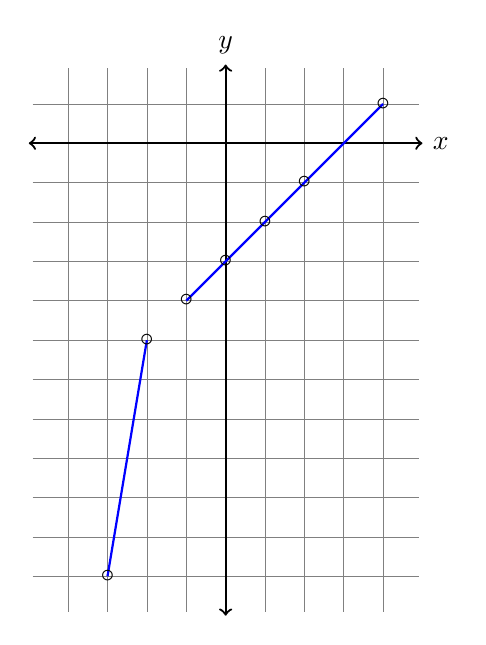
\begin{tikzpicture}[scale=0.5]
            \draw[step=1,gray,very thin] (-4.9,-11.9) grid (4.9,1.9);
            \draw[<->,thick] (-5, 0) -- (5, 0) node[right] {$x$};
            \draw[<->,thick] (0, -12) -- (0, 2) node[above] {$y$};
            
            \draw[domain=-1:4, smooth, variable=\x, thick, blue] plot ({\x}, {\x-3});
            \draw[domain=-3:-2, smooth, variable=\x, thick, blue] plot ({\x}, {6*\x+7});

            \foreach \Point in {(-3,-11), (-2,-5), (-1,-4), (0,-3), (1,-2), (2,-1), (4, 1)}{
                \node at \Point {$\circ$};
            }
        \end{tikzpicture}
    \end{center}
\end{document}
